\normalsize

\title{Assignment 2 Write-Up}
\author{Mukesh Taank}
\date{May 8, 2020}

\begin{document}

\maketitle

\section*{Question 1}
sentence.
sentence.
snetnene.

\section*{Question 2}

This question deals with looking at the SIR model, which is a simple mathematical model of disease spread in a population. 
We are given a set of ordinary differential equations by which this spread is modelled by. 
Using the given initial conditions and differential equations, I was able to use an ODE integrator to solve for the $S$, $I$ and $R$ functions to get their relations with respect to time.
One thing that needed to be done first was to put realistic values for the parameters \beta and \gamma. 
\beta represents the rate of the spread of infection per contact between infected and non-infected per unit time.
\gamma represents the rate at which the infected recover per unit time.
From this, I can find reasonable values for \beta and \gamma. 
Realistic values for \beta and \gamma are between 0 and 1. 
If we assume beta is, for example, 0.5, then this is saying that the disease is spread through 1 meeting between the infected and non-infected every 2 days. 
If we assume gamma is, for example, 0.5, then this is saying one person will recover every 2 days. 
I used the built-in function in SciPy: scipy.integrate.odeint().
When I solved the system of ODEs and finally got my solution functions, I then plotted them onto one graph using varying values for \gamma and \beta.
The following figures show the plots of $S(t)$, $I(t)$ and $R(t)$ with different values of \beta and \gamma.

\begin{figure}
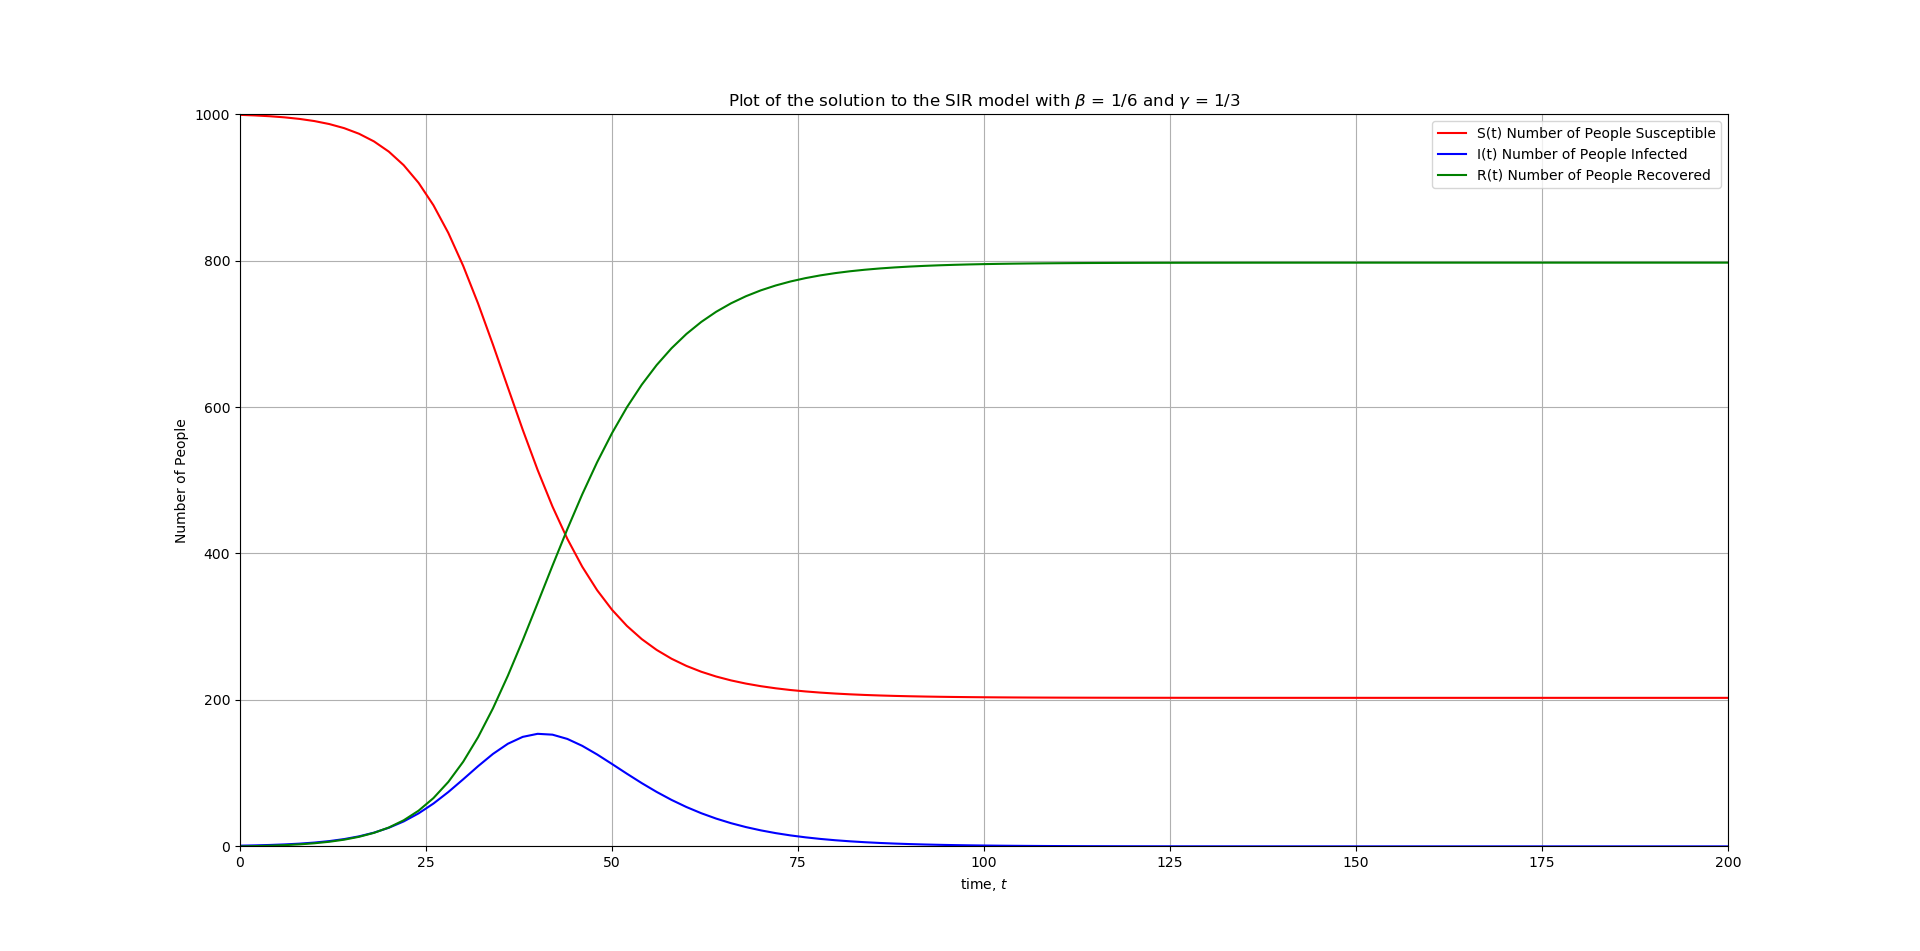
\includegraphics {Q2_plot1.png}
\caption{Plot of the solution functions; $S(t)$, $I(t)$ and $R(t)$ over time, with \beta = 1/6 and \gamma = 1/3.}
\label{fig:figureOfSIRPlot}
\end{figure}

\begin{figure}
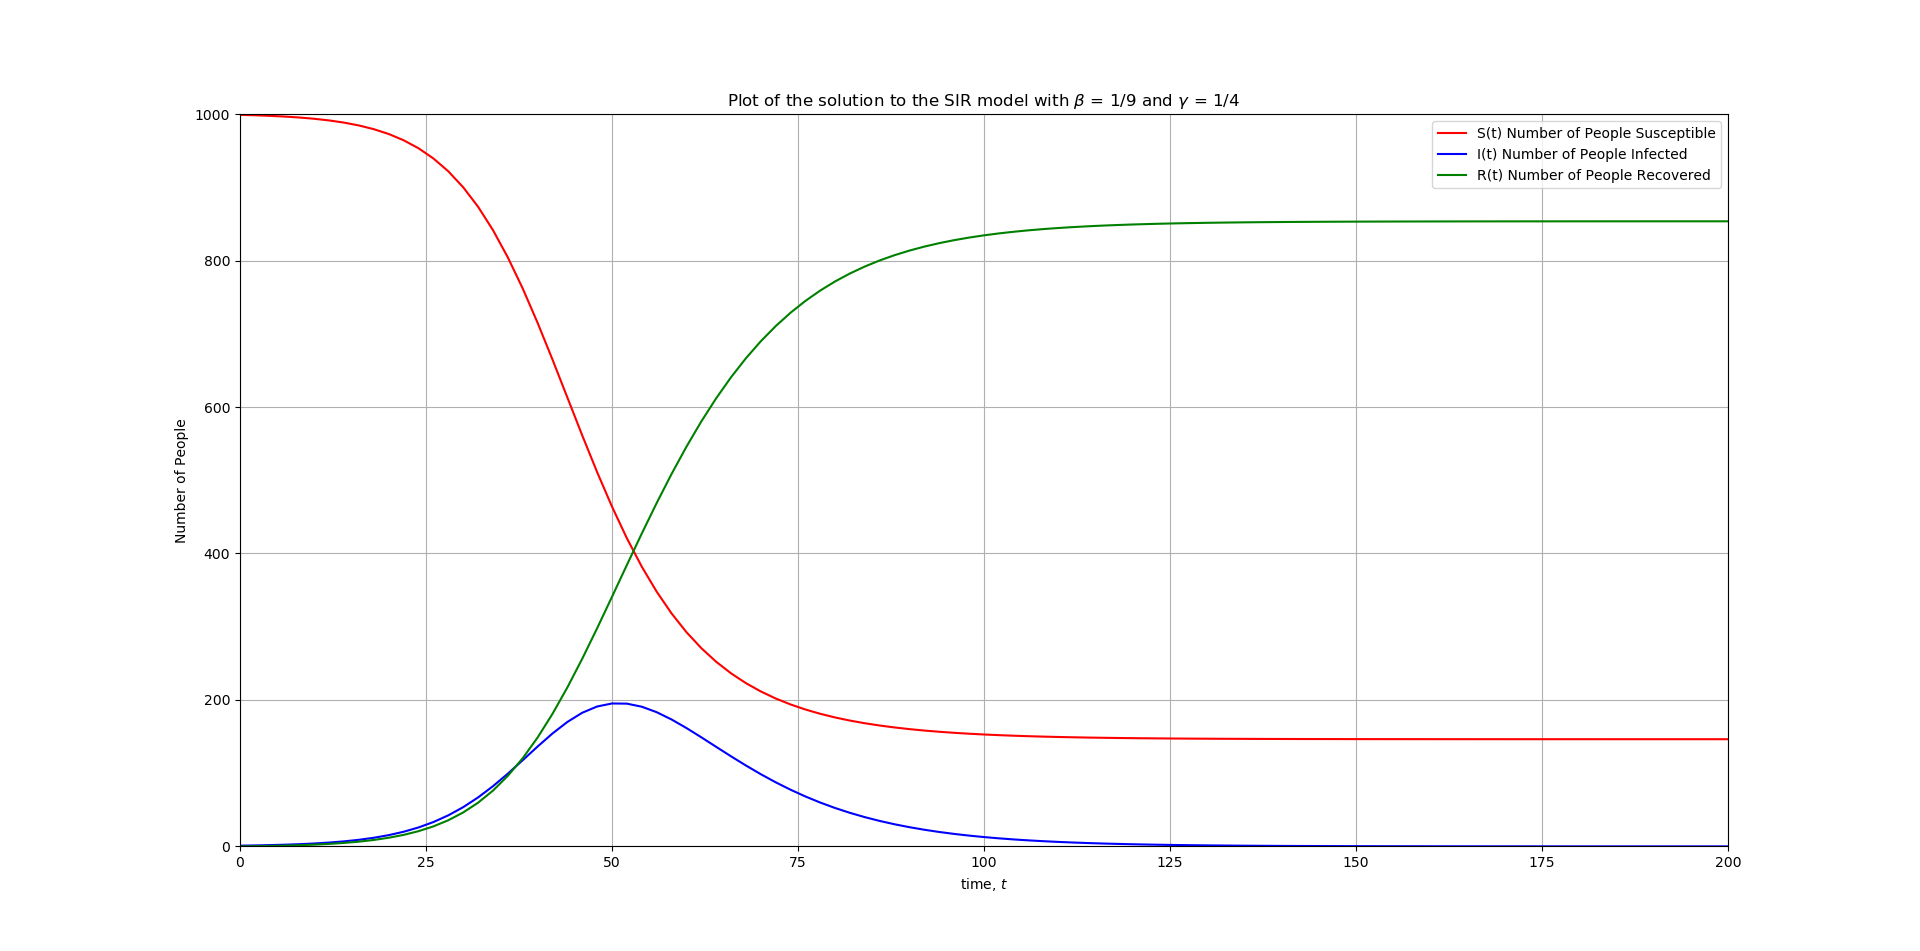
\includegraphics {Q2_plot2.png}
\caption{Plot of the solution functions; $S(t)$, $I(t)$ and $R(t)$ over time, with \beta = 1/9 and \gamma = 1/4.}
\label{fig:figureOfSIRPlot}
\end{figure}

\begin{figure}
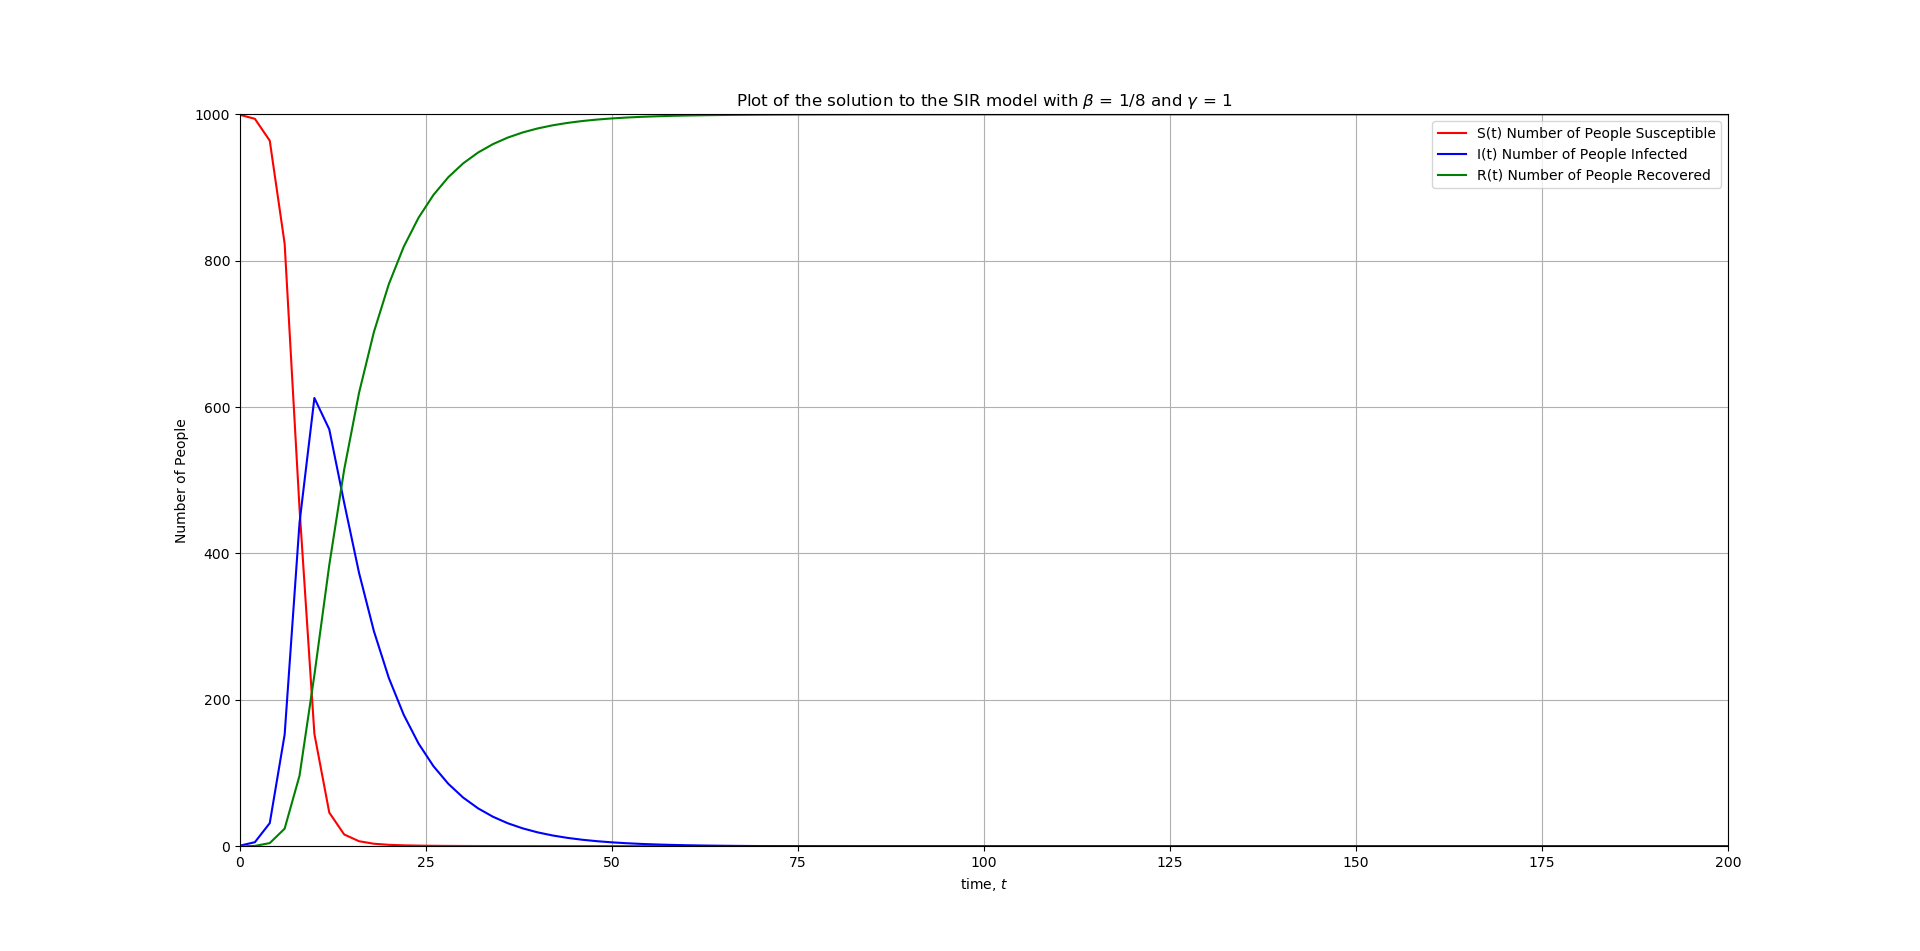
\includegraphics {Q2_plot3.png}
\caption{Plot of the solution functions; $S(t)$, $I(t)$ and $R(t)$ over time, with \beta = 1/8 and \gamma = 1.}
\label{fig:figureOfSIRPlot}
\end{figure}

\begin{figure}
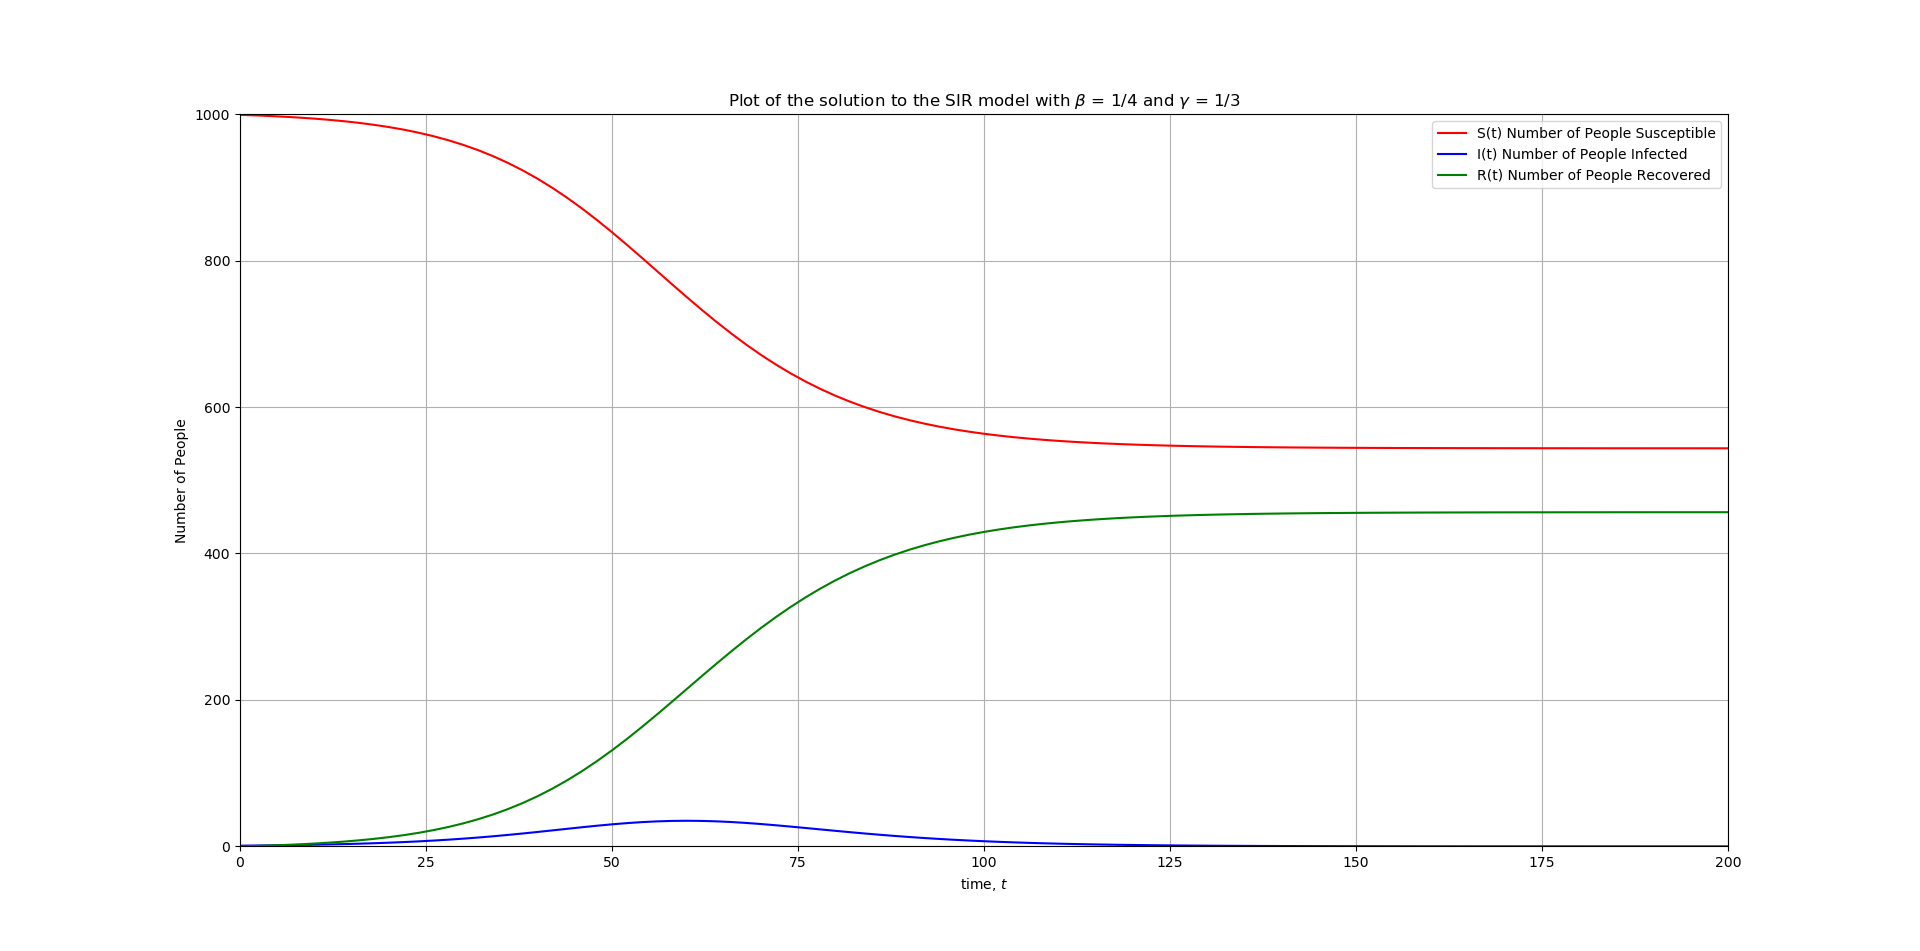
\includegraphics {Q2_plot4.png}
\caption{Plot of the solution functions; $S(t)$, $I(t)$ and $R(t)$ over time, with \beta = 1/4 and \gamma = 1/3.}
\label{fig:figureOfSIRPlot}
\end{figure}


\end{document}
